\documentclass[aps,reprint,prl]{revtex4-1}
\usepackage{graphicx}  % needed for figures
\usepackage{dcolumn}   % needed for some tables
\usepackage{bm}        % for math
\usepackage{amssymb}   % for math
\usepackage{url}
\usepackage{hyperref}

\begin{document}
\title{Cosmology Problem Set 1}
\author{Bismayan Chakrabarti}
\author{Steven Kaplan}
\affiliation{Department of Physics and Astronomy, Rutgers, The State University of New Jersey, 136 Frelinghuysen Road, Piscataway, New Jersey 08854, USA}

\begin{abstract}
Insert an abstract here. Some sort of summary of the theme of all the problems? Think about this.
\end{abstract}

\maketitle

\section*{The Friedmann Equation}
We need some sort of derivation ("Newtonian") or explanation where this comes from (GR).
\begin{equation}
\left(\frac{\dot{a}}{a}\right)^2=\frac{8\pi G}{3}\rho-\frac{k}{a^2}
\end{equation}
\section*{The Einstein-de Sitter Universe}
%Find a way to cite http://www.nicadd.niu.edu/~bterzic/PHYS652/Lecture_05.pdf
Here, $\Omega_{m,0}=1$ since the universe is matter dominated, and $k=0$ because the universe is flat.  The Friedmann equation thus reduces to
\begin{equation}
\left(\frac{\dot{a}}{a}\right)^2=\frac{8\pi G}{3}\rho
\end{equation}
Dodelson shows that conserved quantities in an expanding universe must follow
\begin{equation}
\frac{\partial \rho}{\partial t} + \frac{\dot{a}}{a}\left[3\rho+3P\right]=0
\end{equation}
In our case, $P$ can reasonably be set to zero.  Using the product rule, we can rearrange the above equation to
\begin{equation}
a^{-3}\left(\frac{\partial}{\partial t}\left[\rho a^3\right]\right)=0
\end{equation}
Since $\frac{\partial}{\partial t}\left[\rho a^{3}\right]=0$, this means that $\rho a^{3}=$ a constant.  We can thus claim that $\rho_m \propto a^{-3}$.

Now, since $\Omega_{m,0}=1$, we know that $\rho_m=\rho_{cr}a^{-3}$.  The Friedmann equation now looks like
$$\left(\frac{\dot{a}}{a}\right)^2=\frac{8\pi G}{3}\rho_{cr}a^{-3}$$
Rearranging terms and splitting up the time derivative leaves us with
$$\sqrt{a}\;da=\sqrt{\frac{8\pi G \rho_{cr}}{3}}\;dt$$
Integrating both sides and using the fact that $a=0$ at the big bang, we get
$$a^{\frac{3}{2}}=\frac{3}{2}\sqrt{\frac{8\pi G \rho_{cr}}{3}}\;t$$
Multiplying through by $a^{\frac{2}{3}}$, we finally arrive at
$$a(t)=\left(6\pi G\rho_{cr}\right)^{\frac{1}{3}}t^{\frac{2}{3}}$$
\begin{figure}[h!]
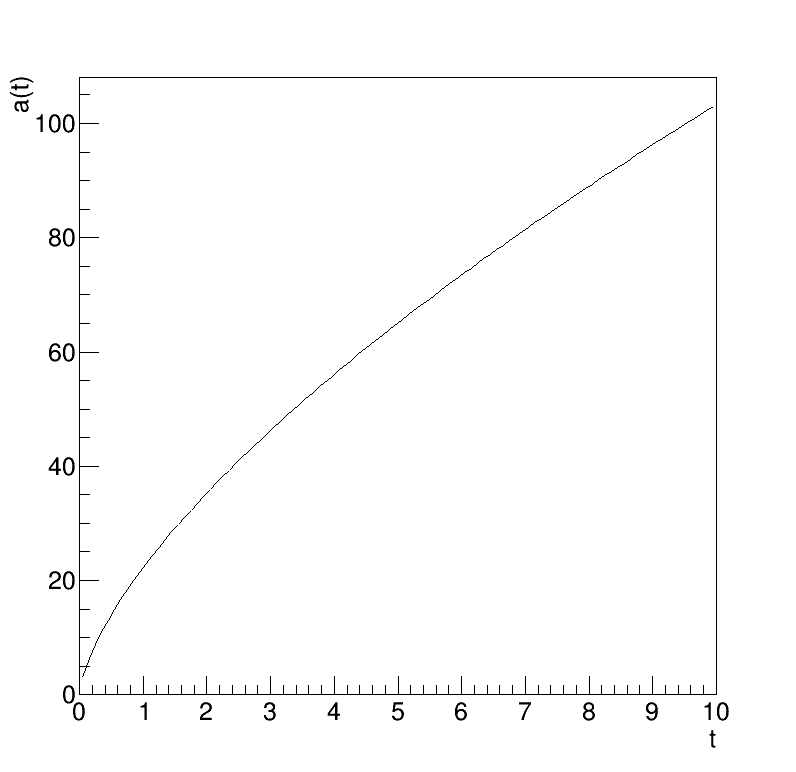
\includegraphics[width=0.5\textwidth]{ps1_plots/a_einstein}
\caption{The time evolution of the scale factor $a$ in an Einstein-de Sitter Universe}
\end{figure}



\end{document}